\documentclass[presentation]{beamer}
\usepackage{../oop-slides}

\title[OOP21: Effective OO Programming]{21 \\ Programmazione Object-Oriented Efficace \\ Principi e ricette}

\begin{document}

\frame[label=coverpage]{\titlepage}

\newcommand{\ecl}{\idepath{p21effective}}


\fr{Outline}{
  \bl{Goal della lezione}{\iz{
  \item Discutere alcuni principi e metodologie di progettazione
  \item Ripassare varie linee guida fornite durante il corso
  \item Illustrarne di nuove largamente accettate
  }}
  \bl{Argomenti}{\iz{
    \item DRY, KISS and SOLID principles
    \item Il testo: J.Block ``Effective Java''
    \item Linee guide di interesse per il corso
    \item Alcuni approfondimenti
  }}
}

\fr{Note generali su questa lezione}{
  \bl{Note:}{\iz{
    \item ri-consolidano vari aspetti già analizzati, ed alcuni nuovi
    \item va vista in prospettiva di una maggiore qualità nello sviluppo del SW
    \item contiene suggerimenti auspicabilmente applicati al progetto d'esame
  }}
}

\frs{5}{SW mal progettato..}{
  \bl{Difetti}{\iz{
    \item rigidità | piccoli cambiamenti richiedono in cascata molte modifiche{\iz{
      \item questo porta a riluttanza a modificare il sistema, incapacità di stimare tempi
    }}
    \item fragilità | cambiamenti ad un modulo/classe, causano il malfunzionamento di altri{\iz{
      \item i cambiamenti fanno diventare il software ``peggiore''
    }}
    \item immobilità | un componente/funzionalità già scritto non è facilmente estraibile/riusabile{\iz{
      \item causato da troppe e inutili dipendenze, si preferisce riscrivere daccapo
    }}
    \item viscosità | deployment e testing sono difficili da realizzare{\iz{
      \item è difficile/costoso verificare il funzionamento corretto di una nuova versione
    }}
    \item complessità | certe porzioni di codice sono più complicate del necessario{\iz{
      \item sono più difficili da capire, modificare, testare 
    }}
    \item ripetitività | certe porzioni di codice sono sostanzialmente duplicate {\iz{
      \item a vari livelli; cioè rende il sistema meno coerente e manutenibile
    }}
    \item opacità | il codice non è comprensibile {\iz{
      \item scarsa documentazione, scarsa leggibilità (nomi variabili, formattazione)
    }}    
  }}
}


\section{Regole base}

\frs{5}{Regole base generali di buona programmazione OOP}{
    \bl{Una lista (fonti eterogeneee)}{\iz{
        \item principio DRY (Don't repeat yourself)
        \item principio KISS (Keep it simple, stupid) -- least surprise
        \item aderire alle convenzione di codice
        \item programmare in inglese
        \item usare nomi (di classe, metodi, campo, variabile) che rivelino in modo cristallino l'intento
        \item usare metodi corti
        \item usare classi corte
        \item ridurre al minimo le assunzioni implicite
        \item ridurre sempre al minimo visibilità e mutabilità
        \item ottimizzare le performance solo se necessario, senza impattare il design
    }}
}

\section{SOLID principles}

\fr{I SOLID principles}{
  \bl{5 principi cardine}{\iz{
    \item SRP: Single responsibility principle{\iz{
      %\item una classe, una sola responsabilità (un motivo per cambiare)
      \item[$\Rightarrow$] ``A class should have one, and only one, reason to change''
    }}
    \item OCP: Open/closed principle{\iz{
      %\item le classi devono essere aperte alle estensioni, ma chiuse alle modifiche
      \item[$\Rightarrow$] ``You should be able to extend a class behavior, without modifying it''
      }}
    \item LSP: Liskov's substitutability principle{\iz{
      %\item le sottoclassi devono essere sostituibili alle sopra-versioni
      \item[$\Rightarrow$] ``Derived classes must be substitutable for their base classes''
    }}
    \item ISP: Interface segregation principle{\iz{
      %\item clienti non devono essere forzati a vedere metodi che non usano
      \item[$\Rightarrow$] ``Make fine grained interfaces that are client specific''
    }}
    \item DIP: Dependency inversion principle{\iz{
      %\item moduli high-level e low-level devono essere comunque disaccoppiati tra loro
      \item[$\Rightarrow$] ``Depend on abstractions, not on concretions''
    }}
  }}
}

\frs{5}{SRP | Single responsibility principle}{
  \bl{``A class should have one, and only one, reason to change''}{\iz{
    \item evitare di costruire classi che gestiscono responsabilità diverse
    \item altrimenti vi saranno più occasioni di doverle modificare
    \item le modifiche rischiano di essere ``poco incapsulate'', andando a toccare uno o più delle varie responsabilità
    \item meglio costruire più classi piccole invece che singole ``enormi'' classi (God class), ma senza nemmeno esagerare
    \item SRP si applica in realtà a metodi, classi e package, a granularità diverse
  }}
  \bl{Esempi visti}{\iz{
    \item MVC: divide in parti diverse le responsabilità M,V,C
    \item Strategy pattern: sposta una strategia fuori dalla classe che la usa (e similmente, Iterator e Observer..)
    \item Esempio negativo: \cil{Stream} (è una API con filosofia ``rich interface''..)
  }}
}

\fr{OCP | Open/closed principle}{
  \bl{``You should be able to extend a class behavior, without modifying it''}{\iz{
    \item costruita/testata una classe, deve essere facile aggiungere funzionalità per estensione, ma non andrebbe più modificata
    \item costruita una classe, la si deve cambiare solo per risolvere dei bug
    \item consente di limitare il bisogno di intaccare codice già testato
    \item[$\Rightarrow$] aderire allo schema Interfaccia - Classi Astratte - Classi Concrete{\iz{
      \item[$\Rightarrow$] classi importanti siano ``nascoste'' da interfacce
      \item[$\Rightarrow$] astrarre dai nomi concreti delle classi per consentire subclassing
      \item[$\Rightarrow$] uso di patterns quali T. Method e Strategy per gestire punti ``caldi''
    }}
      
  }}
  \bl{Esempi visti}{\iz{
    \item Gerarchia collections (\cil{Set}, \cil{AbstractSet}, \cil{HashSet} vs \cil{TreeSet}){\iz{
      \item I clienti si riferiscono perloppiù a \cil{Set}, senza dipendenze sul codice
      \item \cil{AbstractSet} consolida codice riusabile fra le varie implementazioni
      \item \cil{HashSet} e \cil{TreeSet} specializzano opportunamente \cil{AbstractSet}
    }}
  }}
}

\frs{10}{LSP | Liskov's substitutability principle}{
  \bl{``Objects of derived classes must be semantically substitutable for their base version''}{\iz{
    \item la classe che estende/implementa una classe/interfaccia deve ottemperare anche al suo contratto di comportamento informalmente specificato
    \item (javac si occupa solo della parte di ``interfaccia'' del contratto)
    \item questo evita di generare malfunzionamenti quando si passa da comportamenti a loro presunte specializzazioni
    \item[$\Rightarrow$] regole da seguire{\iz{
      \item[$\Rightarrow$] leggere/scrivere documentazione di interfacce e classi
      \item[$\Rightarrow$] non lanciare eccezioni (unchecked) inaspettate
      \item[$\Rightarrow$] non violare regole supposte valide dalla classe/interfaccia base
      \item[$\Rightarrow$] non portare a side-effect inaspettati
      \item[$\Rightarrow$] non stravolgere il funzionamento logico di un metodo in caso di override
    }}
      
  }}
  \bl{Esempi visti}{\iz{
    \item \cil{Iterator.next} deve lanciare una eccezione oltre i limiti
    \item \cil{Object.equals} richiede vari controlli, ad esempio quello sul \cil{null}
    \item \cil{Collection.addAll} non dovrebbe modificare l'argomento
  }}
}

\frs{1}{ISP | Interface segregation principle}{
  \bl{``Make fine grained interfaces that are client specific''}{\iz{
    \item le classi non vanno forzate ad avere (o dipendere da) metodi che non servono
    \item ove possibile, si costruiscano interfacce specifiche per le richieste di ogni tipologia di cliente, con solo i metodi usati{\iz{
      \item[$\Rightarrow$] non avere interfacce con molti metodi
      \item[$\Rightarrow$] ristrutturarle in gerarchie con le tipologie più comunemente richieste
      \item[$\Rightarrow$] se una classe ha due clienti diversi, forse dovrebbe avere due interfacce
    }}
    \item La main GUI di una applicazione ha una interfaccia verso il controller, e una verso una sotto-GUI
  }}
  %\bl{Esempi visti: gerarchia interfacce \cil{Collection}}{
  %  \centering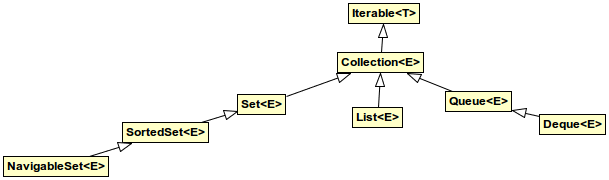
\includegraphics[width = 0.7\textwidth]{\ecl/collection-hierarchy.png}
  %}
}

\frs{1}{DIP | Dependency Inversion Principle}{
  \bl{``Depend on abstractions, not on concretions''}{\iz{
    \item una variante di (o accoppiamento a) OCP
    \item una classe non sia dipendenti da un aspetto implementativo estraibile, bensì..
    \item tale aspetto sia astratto da una interfaccia da cui si dipende
    \item regole da seguire{\iz{
      \item[$\Rightarrow$] creare una barriera di astrazione fra classi che lavorano a livello diverso o che appartengono a componenti logiche diverse
    }}
    \item limitare al massimo i casi di classi che dipendono tra loro
  }}
  \bl{Esempi visti}{\iz{
    \item gerarchia \cil{Collection}, \cil{Device} (domotica), \cil{Comparable},..
  }}
  \centering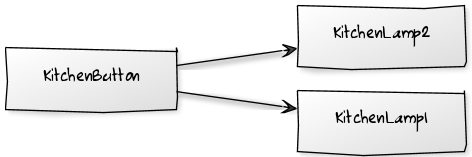
\includegraphics[width = 0.35\textwidth]{img/DIP1.png}~
  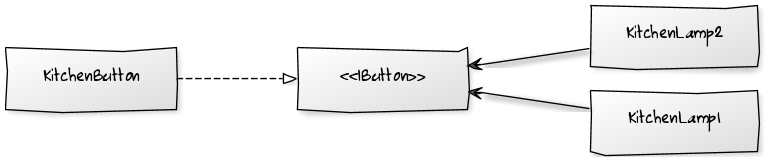
\includegraphics[width = 0.6\textwidth]{img/DIP2.png}
}

\fr{Riassunto: SOLID principles in Java}{
  \bl{5 principi cardine}{\iz{
    \item SRP: Single responsibility principle{\iz{
      \item[$\Rightarrow$] tenere le classi ``piccole'' e coerenti 
    }}
    \item OPC: Open/closed principle{\iz{
      \item[$\Rightarrow$] fattorizzare codice funzionante in classi estendibili (astratte o non)
      }}
    \item LSP: Liskov's substitutability principle{\iz{
      \item[$\Rightarrow$] obbedire anche al contratto (sottointeso) di una classe/interfaccia base
    }}
    \item ISP: Interface segregation principle{\iz{
      \item[$\Rightarrow$] costruire gerarchie fatte di interfacce ``piccole'', coerenti e utili
    }}
    \item DIP: Dependency inversion principle{\iz{
      \item[$\Rightarrow$] dipendere da interfacce, non dalle loro implementazioni 
    }}
  }}
}


\section{Linee guida di programmazione efficace}


\fr{Linee guida di programmazione efficace}{
  \bl{Alcuni elementi}{\iz{
    \item Sono indicazioni operative su come comportarsi in certe situazioni di programmazione, con lo scopo di ottenere una programmazione più efficace e moderna (maggior prestazioni, flessibilità, leggibilità)
    \item Sono disgiunte (anche se non del tutto) da altri aspetti correlati: convenzioni sul codice, principi, pattern, regole di ``clean coding''
    \item Spunto tratto da: J.Block ``Effective Java''
  }}
  \bl{In questa lezione}{\iz{
    \item Illustreremo varie linee guida
    \item Ne approfondiremo qualcuna
    \item Da usare ove possibile all'esame
    \item Da usare in futuro
  }}
  
}

\frs{5}{Effective Java, 2nd edition}{
  \bl{Struttura del testo}{\iz{
    \item 78 item, ossia 78 suggerimenti, numerati
    \item divisi in 10 capitoli (creazione/distruzione oggetti, metodi comuni a tutti gli oggetti, classi/interfacce, generici, enum/annotazioni, metodi, programmazione, eccezioni, concorrenza, serializzazione)
    \item tutti condivisibili, ne approfondiremo un sottoinsieme
  }}
  \bl{Ogni linea guida descrive}{\iz{
    \item la situazione(i) in cui si usa
    \item cosa è opportuno fare in quei casi
    \item motivazioni e vantaggi/svantaggi
  }}
  \bl{Di interesse per noi}{\iz{
    \item un sottoinsieme di linee guida
    \item moltissime già incontrate
  }}
}

\frs{5}{La parte di catalogo che ci concerne (1/3)}{
    \bl{Creating and destroying objects}{\iz{
	\item \alert{Consider static factory methods instead of constructors}
	\item \alert{Consider a builder when faced with many constructor parameters}
	\item \alert{Enforce the singleton property with a private constructor or an enum type}
	\item \alert{Enforce noninstantiability with a private constructor}
    }}
    \bl{Methods common to all objects}{\iz{
	\item \alert{Obey the general contract when overriding \cil{equals}}
	\item \alert{Always override \cil{hashCode} when you override \cil{equals}}
	\item \alert{Always override \cil{toString}}
    }}
    \bl{Classes/interfaces}{\iz{
	\item \alert{Minimize the accessibility of classes and members}
	\item \alert{In public classes, use accessor methods, not public fields}
	\item \alert{Minimize mutability}
	\item \alert{Favor composition over inheritance}
	\item \alert{Design and document for inheritance or else prohibit it}
	\item \alert{Prefer interfaces over abstract classes}
    }}
}

\frs{5}{La parte di catalogo che ci concerne (2/3)}{
    \bl{Generics}{\iz{
	\item \alert{Don’t use raw types in new code}
	\item \alert{Eliminate unchecked warnings}
	\item \alert{Prefer lists to arrays}
    }}
    \bl{Enum and annotations}{\iz{
	\item \alert{Use enums instead of int constants}
	\item \alert{Use \cil{EnumMap} instead of ordinal indexing}
	\item \alert{Consistently use the \cil{Override} annotation}
    }}
    \bl{Methods}{\iz{
	\item \alert{Check parameters for validity}
	\item \alert{Make defensive copies when needed}
	\item \alert{Write doc comments for all exposed API elements}
    }}
}

\frs{5}{La parte di catalogo che ci concerne (3/3)}{
    \bl{General Programming}{\iz{
	\item \alert{Minimize the scope of local variables}
	\item \alert{Prefer for-each loops to traditional for loops}
	\item \alert{Know and use the libraries}
	\item \alert{Avoid float and double if exact answers are required}
	\item \alert{Prefer primitive types to boxed primitives}
	\item \alert{Avoid strings where other types are more appropriate}
	\item \alert{Beware the performance of string concatenation}
	\item \alert{Refer to objects by their interfaces}
	\item \alert{Adhere to generally accepted naming conventions}
    }}
    \bl{Exceptions}{\iz{
	\item \alert{Use exceptions only for exceptional conditions}
	\item \alert{Use checked exceptions for recoverable conditions and runtime exceptions for programming errors}
	\item \alert{Avoid unnecessary use of checked exceptions}
	\item \alert{Favor the use of standard exceptions}
	\item \alert{Include failure-capture information in detail messages}
    }}
}

\subsection{Classi e metodi comuni}

\frs{1}{Creating and destroying objects}{
    \bl{Creating and destroying objects}{\iz{
	\item \alert{Consider static factory methods instead of constructors}
	\item \alert{Consider a builder when faced with many constructor parameters}
	\item Enforce the singleton property with a private constructor or an enum type
	\item Enforce noninstantiability with a private constructor
    }}
    \bl{Static factory, confronto con l'uso di costruttori}{\iz{
       \item[$+$] possiamo dargli un nome espressivo
       \item[$+$] possiamo avere più costruzioni diverse a parità di signature
       \item[$+$] possiamo istanziare una specializzazione
       \item[$-$] problematico con strutture di ereditarietà
       \item[$-$] difficile distinguere i factory dagli altri metodi, valutare di spostarli
    }}
    \bl{Consider a builder when faced with many constructor parameters}{\iz{
      \item Quando la costruzione è complessa, e favorisce un approccio step-by-step
    }}
}

\frs{5}{Creating and destroying objects: sui singleton}{
    \bl{Creating and destroying objects}{\iz{
	\item Consider static factory methods instead of constructors
	\item Consider a builder when faced with many constructor parameters
	\item \alert{Enforce the singleton property with a private constructor or an enum type}
	\item Enforce noninstantiability with a private constructor
    }}
    \bl{Enforce the singleton property with a private constructor or an enum type}{\iz{
        \item Come sappiamo i singleton abbiano costruttore privato
        \item Block suggerisce l'uso di una \cil{enum} a singolo valore \cil{SINGLETON} per realizzare un singleton{\iz{
	  \item Gestisce bene serializzazione e thread-safety
	  \item Forza una visione, peraltro ragionevole, di una \cil{enum} come collezione di un insieme finito di oggetti (nella fattispecie, 1)
	}}
    }}
}

\fr{Singleton con \Cil{enum}}{
  \sizedrangedcodet{\ssmall}{3}{100}{\ecl/singleton/Log.java}
}

\frs{5}{Creating and destroying objects: costruttori privati}{
    \bl{Creating and destroying objects}{\iz{
	\item Consider static factory methods instead of constructors
	\item Consider a builder when faced with many constructor parameters
	\item Enforce the singleton property with a private constructor or an enum type
	\item \alert{Enforce noninstantiability with a private constructor}
    }}
    \bl{Enforce noninstantiability with a private constructor}{\iz{
        \item Ricordarsi di nascondere i costruttori in classi ``helper''
        \item Vedi classi \cil{java.lang.Math}, \cil{java.util.Collections}
    }}
}


\frs{5}{Methods common to all objects}{
    \bl{Methods common to all objects}{\iz{
	\item \alert{Obey the general contract when overriding \cil{equals}}
	\item \alert{Always override \cil{hashCode} when you override \cil{equals}}
	\item \alert{Always override \cil{toString}}
    }}
        \bl{Alcuni fatti riepilogativi di quanto già visto}{\iz{
	\item \cil{equals} è usato in tutto il Collection framework (\cil{Collection.contains/remove}, \cil{Map.get})
	\item \cil{hashCode} è usato in \cil{HashSet} e \cil{HashMap}
	\item è opportuno definirli (bene!) in coppia e farli lavorare sullo stesso set di campi, perché è facile cambiare collezione così che serva l'hashcode
	\item è opportuno ri-definire \emph{sempre} \cil{toString}, anche a fini di debug, esponendo le info pubbliche rilevanti
	\item l'uso (informato) di Eclipse è molto utile
	\item attenzione alla semantica intesa quando servono implementazioni ad-hoc (\cil{java.lang.Object})
    }}

}

\frs{5}{Classes/interfaces}{
    \bl{Classes/interfaces}{\iz{
	\item \alert{Minimize the accessibility of classes and members}
	\item \alert{In public classes, use accessor methods, not public fields}
	\item \alert{Minimize mutability}
	\item \alert{Favor composition over inheritance}
	\item \alert{Design and document for inheritance or else prohibit it}
    }}
    ..prossime slide
}

\fr{Classi e interfacce: minimize accessibility}{
    \bl{Minimize the accessibility of classes and members: filosofia}{
	Per il principio dell'information-hiding, e per evitare di influenzare molte classi con delle modifiche, si renda ogni proprietà (classe, metodo, campo) visibile il meno possibile
    }
    \bl{Fatti principali}{\iz{
	\item Classi ad uso ``interno'' di una libreria o applicazione siano package-private, ossia non le si dichiari pubbliche
	\item Classi usate solo da un'altra classe \cil{C}, vengano innestate private in \cil{C} (oop12) -- senza eccessi
	\item Limitare visibilità di campi/metodi (\cil{private}, \cil{protected}, \cil{public})
	\item L'uso del livello package-private è avanzato, da usare documentando
	\item L'esposizione ``pubblica'' di una proprietà è un fatto ``rilevante''
    }}
}

\fr{Classi e interfacce: don't use public fields}{
    \bl{In public classes, use accessor methods, not public fields: filosofia}{
	La struttura di un oggetto è un aspetto implementativo, e come tale suscettibile di modifiche successive che non devono toccare i clienti
    }
    \bl{Fatti principali}{\iz{
	\item L'esistenza di un getter o setter non implica l'esistenza di un campo{\iz{
	  \item Una classe che rappresenta uno slot temporale in una agenda appuntamenti avrebbe getter e setter per ora e minuto di inizio dello slot, ma quale campo usereste?
	}}
	\item Alcuni ritengono che in classi non pubbliche sia accettabile avere campi non privati, per avere codice più compatto, ma questo pone comunque vincoli a modifiche successive{\iz{
	  \item È sconsigliato, ma non è un errore
	}}
	\item Anche i campi \cil{protected} sono sconsigliati
    }}
}

\frs{5}{Classi e interfacce: minimize mutability}{
    \bl{Minimize mutability: filosofia}{
	Cercare di rendere meno mutabile possibile il codice: ciò rende il codice più semplice, evita errori e interferenze fra il lavoro dei clienti
    }
    \bl{Fatti principali}{\iz{
	\item Campi e variabili siano finali se non serve esplicitamente il contrario
	%\item Metodi e classi siano finali se si vuole prevenire la loro specializzazione
	\item Classi immutabili hanno campi finali che sono a loro volta immutabili
	\item Invece di metodi ``mutators'', si usi l'approccio funzionale{\iz{
	  \item il metodo torni un nuovo oggetto, senza modificare \cil{this}
	}}
	\item Esempi: \cil{String}, \cil{Integer}, \cil{Date}.. perché?
	\item Vantaggi:{\iz{
	  \item classi più semplici
	  \item classi thread-safe
	  \item oggetti facilmente ``sharable'' (p.e.: costanti)
	  \item ottimizzazioni (flighweight, caching)
	}}
	
    }}
}

\fr{Un esempio di design avanzato di una API: Complex}{
  \bl{Astrazione numero Complesso: funzionalità}{\iz{
    \item costruibile sia in coordinate polari che cartesiane
    \item astrazione ovviamente immutabile
    \item metodi per cambiare coordinate (senza mutabilità)
    \item approccio completamente ``funzionale''
  }}
  \bl{Dettagli interni}{\iz{
    \item interfaccia senza metodi default
    \item interfaccia con static factory
    \item costruzione oggetti con riuso della costante ``zero''
    \item classe astratta per fattorizzare codice comune
    \item codice implementativo package-protected
    \item implementazaione cartesiana-polare scelta ``dinamicamente''
  }}
}

\fr{\Cil{Complex}: UML completo}{
\begin{center}
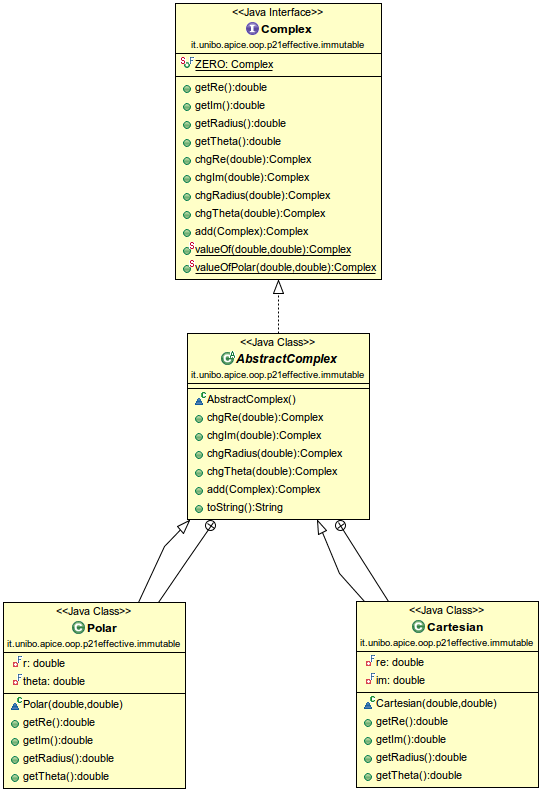
\includegraphics[height= 0.8\textheight]{\ecl/complex.png}
\end{center}
}

\fr{Interfaccia \Cil{Complex}: 1/2}{
  \sizedrangedcodet{\ssmall}{3}{25}{\ecl/immutable/Complex.java}
}

\fr{Interfaccia \Cil{Complex}: 2/2}{
  \sizedrangedcodet{\ssmall}{26}{100}{\ecl/immutable/Complex.java}
}

\fr{\Cil{AbstractComplex}}{
 \vspace{-5pt}
 \sizedrangedcodet{\tiny}{3}{35}{\ecl/immutable/AbstractComplex.java}
}

\fr{\Cil{AbstractComplex.Cartesian}}{
 \vspace{-5pt}
 \sizedrangedcodet{\tiny}{37}{66}{\ecl/immutable/AbstractComplex.java}
}

\fr{\Cil{AbstractComplex.Polar}}{
 \vspace{-5pt}
 \sizedrangedcodet{\tiny}{68}{120}{\ecl/immutable/AbstractComplex.java}
}

\fr{\Cil{UseComplex}}{
 \sizedrangedcodet{\ssmall}{6}{120}{\ecl/immutable/UseComplex.java}
}


\frs{5}{Classi e interfacce: favour composition over inheritance}{
    \bl{Favour composition over inheritance: filosofia}{
	In molti contesti l'ereditarietà (fra classi) non è la migliore strategia di riuso, meglio usare delegazione, ossia con una decorazione
    }
    \bl{Fatti principali}{\iz{
	\item L'ereditarietà funziona bene solo se il programmatore ha il controllo di entrambe le classi
	\item Non c'è vero incapsulamento fra una classe e la sua sotto-classe{\iz{
	  \item modifiche apparentemente innocue nella sopra-classe potrebbero compromettere il funzionamento della sotto-classe
	}}
	\item Spesso si vuole ereditare parte del codice, non tutto
	\item Spesso l'aspetto is-a della relazione di ereditarietà è secondario
	\item In molti linguaggi (Java), l'erediterietà è ``singola''
	\item Valutare l'uso di un approccio a decorazione
	\item Eclipse fornisce anche un modo veloce di creare ``delegazione''
    }}
}

\fr{L'esempio \Cil{Counter}: UML completo}{
\begin{center}
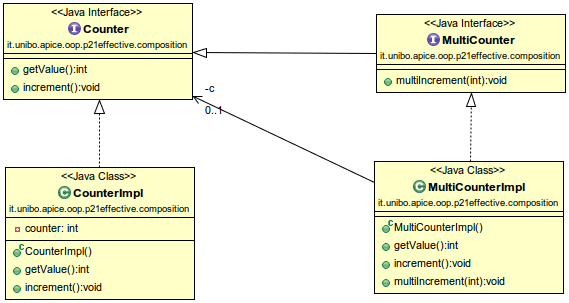
\includegraphics[height= 0.6\textheight]{\ecl/composition.png}
\end{center}
}

\fr{\Cil{Counter} e \Cil{MultiCounter}}{
  \sizedrangedcodet{\ssmall}{3}{25}{\ecl/composition/Counter.java}
  \sizedrangedcodet{\ssmall}{3}{25}{\ecl/composition/CounterImpl.java}
  \sizedrangedcodet{\ssmall}{3}{25}{\ecl/composition/MultiCounter.java}
}

\fr{Implementazione \Cil{MultiCounterImpl} via composizione}{
  \sizedrangedcodet{\ssmall}{3}{25}{\ecl/composition/MultiCounterImpl.java}
}


\fr{Classi e interfacce: Prefer interfaces to abstract classes}{
    \bl{Prefer interfaces to abstract classes: filosofia}{
	Quando va creato un tipo di dato relativamente ad un contratto è molto meglio usare una \cil{interface} piuttosto che una classe astratta (con tutti metodi astratti).
    }
    \bl{Fatti principali}{\iz{
	\item È molto più facile implementare una interfaccia che estendere una classe, grazie alla possibilità di ereditarietà multipla
	\item In Java il pattern adapter si realizza facilmente per adattarsi ad una interfaccia (oop20){\iz{
	\item Es.: è meglio adattarsi ad un \cil{Runnable} o ad un \cil{Thread}?
	}}
	\item I \cil{default} di Java 8+ rendono le interfacce più simili alle classi astratte, e quindi allargano la possibilità di usare le interfacce
    }}
}

\subsection{Tipi e metodi}

\frs{5}{Generics}{
    \bl{Generics}{\iz{
	\item \alert{Don’t use raw types in new code}
	\item \alert{Eliminate unchecked warnings}
	\item \alert{Prefer lists to arrays}
    }}
    ..prossime slide
}

\fr{Generics: Don't use raw types in new code}{
    \bl{Don't use raw types in new code: filosofia}{
	È possibile usare una classe generica come se non lo fosse, ma è sconsigliato in codice ``nuovo'': è solo tollerato in codice versione pre-Java 5.
    }
    \bl{Fatti principali}{\iz{
	\item È possibile scrivere: \cil{List list = new ArrayList();}
	\item Più o meno è come lavorare con \cil{List<Object>}.. non si hanno i vantaggi della genericità
	\item Il compilatore segnala un warning
	\item Lavorare con i raw type è severamente sconsigliato
    }}
}

\fr{Generics: Eliminate unchecked warnings}{
    \bl{Eliminate unchecked warnings: filosofia}{
	Non si devono tollerare i warning, perché ci si abitua ad averne, e quindi ad ignorare i warning segnalati dal compilatore.
    }
    \bl{Fatti principali}{\iz{
	\item Esempi: uso di raw type, conversioni di tipo con generici, etc.. (oop9)
	\item A volte non si possono evitare, in qual caso usiamo l'annotazione \cil{SuppressWarning} (oop9)
	\item Se si possono evitare, evitiamoli
	\item Discorso analogo per ogni altro warning segnalato dal compilatore
    }}
}

\fr{Generics: Prefer lists to arrays}{
    \bl{Prefer lists to arrays: filosofia}{
	Gli array sono una specie di tipo generico, ma per motivi di legacy non si integrano molto bene con tutto il resto della genericità. Quindi, è in generale meglio usare il tipo generico più simile: le \cil{java.util.List}
    }
    \bl{Fatti principali}{\iz{
	\item Gli array sono trattati ``erroneamente'' come covarianti (oop9,p58)
	\item Non si integrano bene: \cil{List<Integer[]>} ok, \cil{List<Integer>[]} no
	\item Agli array si può chiedere il tipo preciso (sono \alert{reificati}), ai generici no
	\item Ok usare array di tipi primitivi per motivi di performance
	\item Ok usare array (\cil{Integer[]}) se siamo certi di non incappare nei problemi di cui sopra
	\item Altrimenti conviene usare le liste, che forniscono anche più operazioni, oppure liste non modificabili (\cil{Collections.unmodifiableList})
	
    }}
}

\frs{5}{Enum and annotations}{
    \bl{Enum and annotations}{\iz{
	\item \alert{Use enums instead of int constants}
	\item \alert{Consistently use the \cil{Override} annotation}
	\item \alert{Use \cil{EnumMap} instead of ordinal indexing}
    }}
    \bl{Ricordiamo:}{\iz{
      \item Le enumerazioni andrebbero usate sempre quando una classe ha un numero finito e noto di oggetti, ossia per modellare insiemi finiti (e noti) di elementi
      \item J.Block addirittura suggerisce di usare le Enum anche al posto dei booleani (e addirittura per il Singleton)
      \item Una struttura frequentemente utile è la mappa da enumerazioni a valori, usare l'implementazione ottimizzata \cil{EnumMap}
    }}
    
}

\fr{\Cil{UseEnumMap}}{
  \sizedrangedcodet{\ssmall}{6}{100}{\ecl/enummap/UseEnumMap.java}
}


\frs{5}{Methods}{
    \bl{Methods}{\iz{
	\item \alert{Make defensive copies when needed}
	\item Check parameters for validity
	\item Write doc comments for all exposed API elements
    }}
    \bl{Getter di campi}{\iz{
      \item Se un campo ha un getter ma non un setter, bisogna accertarsi che modificando l'oggetto tornato dal getter non si modifichi il campo
      \item Se c'è questo pericolo (gli oggetti dei campi non sono immutabili) bisogna fare copie difensive
      \item Si clona l'oggetto e si restituisce la versione clonata
      \item Con le collezioni si può usare una vista non modificabile -- nelle API di Java sono realizzate mediante ``composizione'' (decorator), ossia \cil{Collections.unmodifiableList}
    }}
}

\fr{\Cil{MyCollection}}{
  \sizedrangedcodet{\ssmall}{5}{100}{\ecl/defensive/MyCollection.java}
}

\fr{Methods: Check parameters for validity}{
    \bl{Check parameters for validity: filosofia}{
	Non sempre si può assumere che un cliente sappia i vincoli che gli input di un metodo debbano soddisfare, quindi è opportuno che un metodo (specialmente se pubblico) effettui i controlli necessari, lanciando eccezioni se necessario.
    }
    \bl{Fatti principali}{\iz{
	\item Aggiungere i controlli necessari spesso porta a penalizzazione in performance, ed è noioso
	\item Nei metodi pubblici è però fondamentale
	\item Si lancino eccezioni ``unchecked'', specialmente se l'errore è dovuto ad una errata lettura della documentazione
	\item Si lancino eccezioni ``checked'' se invece l'errore non era facilmente intercettabile dal cliente
    }}
}

\fr{Methods: Write doc comments for all exposed API elements}{
    \bl{Write doc comments for all exposed API elements}{
    È necessario mettere commenti JavaDoc su tutti i metodi pubblici
	}
    \bl{Fatti principali}{\iz{
	\item Sicuramente nelle interfacce
	\item Nei metodi con override solo se l'override richiede ulteriore commento
	\item Tendenzialmente non mettere commenti nei corpi, meglio programmare rivelando l'intento
    }}
}
\subsection{Programmazione varia}

\frs{5}{General Programming}{
    \bl{General Programming}{\iz{
	\item \alert{Minimize the scope of local variables}
	\item \alert{Prefer for-each loops to traditional for loops}
	\item Know and use the libraries
	\item Avoid float and double if exact answers are required
	\item Prefer primitive types to boxed primitives
	\item Avoid strings where other types are more appropriate
	\item Beware the performance of string concatenation
	\item Refer to objects by their interfaces
	\item Adhere to generally accepted naming conventions
    }}
    \bl{Discussione}{\iz{
      \item Definire una variabile quando serve, non ad inizio metodo!{\iz{
	\item minimizza errori e aumenta la leggibilità
	}}
      \item La dichiaratività rende il codice più comprensibile e chiaro, quindi:{\iz{
	\item meglio metodo \cil{forEach}, poi costrutto for-each, poi il \cil{for} classico
      }}
    }}
}

\fr{General programming: Know and use the libraries}{
    \bl{Know and use the libraries: filosofia}{
	Le librerie fornite incapsulano funzionalità note a tutti e ben funzionanti. Usarle è \alert{molto} meglio che riscriversi pezzi di codice da soli.
    }
    \bl{Fatti principali}{\iz{
	\item Il codice che usa librerie è di migliore qualità: più leggibile, comprensibile, corretto, performante.
	\item Conoscere le librerie evita di ``reinventare la ruota''
	\item Librerie importanti (in \cil{java.lang}, \cil{java.util}, \cil{java.util.stream}, \cil{java.io} e \cil{javax.swing}), anche all'esame:{\iz{
	    \item \cil{Math}, \cil{Collections}, \cil{Arrays}, \cil{Collection}, \cil{Iterator}, \cil{List}, \cil{Set}, \cil{Object}, \cil{Integer}, \cil{InputStream}, \cil{JFrame}, \cil{JPanel}..
	}}
	\item ..ma non cercate librerie per ogni cosa vi serva: assicuratevi di non diventarne dipendenti al punto di non saper più realizzare niente da soli
    }}
}

\frs{5}{General Programming}{
    \bl{General Programming}{\iz{
	\item Minimize the scope of local variables
	\item Prefer for-each loops to traditional for loops
	\item Know and use the libraries
	\item \alert{Avoid float and double if exact answers are required}
	\item \alert{Prefer primitive types to boxed primitives}
	\item \alert{Avoid strings where other types are more appropriate}
	\item \alert{Beware the performance of string concatenation}
	\item Refer to objects by their interfaces
	\item \alert{Adhere to generally accepted naming conventions}
    }}
    \bl{Discussione}{\iz{
      \item Ricordarsi i problemi di precisione dei float e double
      \item I primitive sono più veloci e espressivi, i boxed servono per la visione ``everything is an object''
      \item Non rappresentate come stringhe valori che modellano concetti diversi
      \item La creazione di stringhe complesse avvenga con \cil{StringBuffer}
      \item Seguite le convenzioni Java.. sempre!
    }}
}


\fr{General programming: Refer to objects by their interfaces}{
    \bl{Refer to objects by their interfaces: filosofia}{
	I clienti di un oggetto percepiscono solo la sua interfaccia. Quindi, ove disponibile, è sempre meglio indicare tipi \cil{interface}: si ha una visione più astratta, meno vincolata all'implementazione, più riusabile, e più aperta ai cambiamenti (si segue il principio DIP)
    }
    \bl{Fatti principali}{\iz{
	\item Nelle proprie gerarchie di oggetti, si cerchino sempre di costruire le interfacce più significative, che denotano i tipi fondamentali di oggetti. (ISP)
	\item Usare interfacce in parametri, tipi di ritorno e variabili/campi
    }}
}


\frs{5}{Exceptions}{
    \bl{Exceptions}{\iz{
	\item Use exceptions only for exceptional conditions
	\item Use checked exceptions for recoverable conditions and runtime exceptions for programming errors
	\item Avoid unnecessary use of checked exceptions
	\item \alert{Favor the use of standard exceptions}
	\item Throw exceptions appropriate to the abstraction
	\item Document all exceptions thrown by each method
	\item Include failure-capture information in detail messages
    }}
}

\fr{Exceptions}{
    \bl{Discussione}{\iz{
	\item Usare appropriatamente le eccezioni unchecked \cil{IllegalArgumentException},  \cil{IllegalStateException}, \cil{NullPointerException}, \cil{IndexOutOfBoundsException}, \cil{UnsupportedOperationException}
	\item Lanciare eccezioni compatibili col livello d'astrazione della classe, catturando quelle di basso livello e rilanciando quelle di alto livello (vedi \cil{AbstractSequentialList.get})
	\item Documentare le eccezioni, dichiarare il \cil{throws} solo per le checked
    }}

}

\fr{Conclusione}{
    \bl{Costruire del buon codice è un mix di vari aspetti}{\iz{
	\item Uso delle convenzioni sulla formattazione del codice
	\item Uso di tecniche di programmazione efficace
	\item Uso di plugin per check di stile o di bug
	\item Uso di pattern di progettazione
	\item Uso efficiente delle risorse disponibili
	\item[$\Rightarrow$] Il tutto richiede esperienza
    }}
    \bl{Dall'OO alla costruzione di software}{\iz{
	\item Quanto visto nel corso ha validità generale per l'Ingegneria Informatica
	\item L'OO è lo stile più usato
	\item Ma le tecniche ed esperienze viste sono cruciali in ogni contesto di progettazione/costruzione di sistemi informatici
    }}
}


\end{document}
